\begin{frame}{Распределение интенсивности МК когерентностей ЯМР}
\vspace{-5mm}
$$ 
G(\tau, \phi) =
\mathrm{Tr}\left\{
   e^{iH_\mathrm{MQ}\tau} e^{i\phi I_z} e^{-iH_\mathrm{MQ}\tau}
   \rho_\mathrm{eq}
   e^{iH_\mathrm{MQ}\tau} e^{-i\phi I_z} e^{-iH_\mathrm{MQ}\tau}
   I_z 
\right\}
$$
\vspace{-5mm}
\begin{columns}
  \column{0.4\textwidth}
  \vspace{-3mm}
  \begin{figure}
    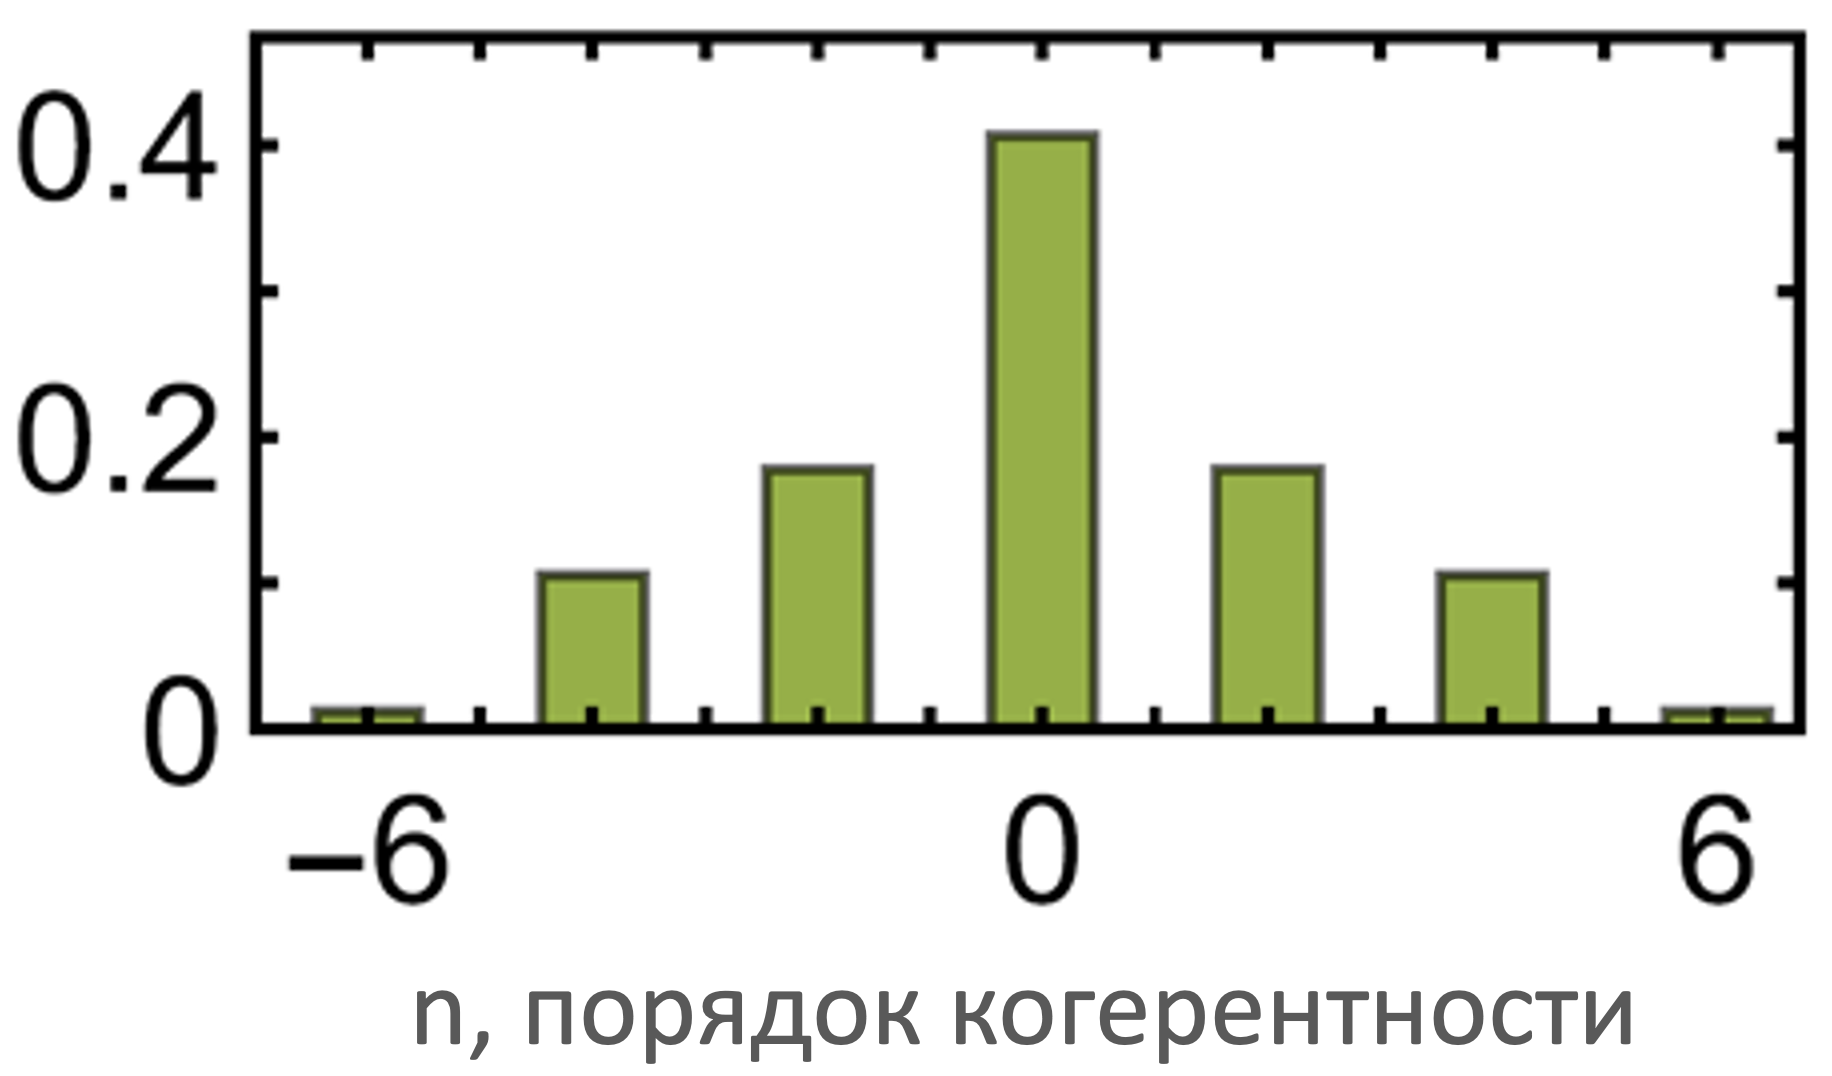
\includegraphics[width=\textwidth]{mq-coherence-intensities-hist.png}
    \caption{$J_{k}$, распределение интенсивности МК когерентностей ЯМР.}
  \end{figure}

  \column{0.5\textwidth}
  \begin{block}{}
    Второй момент (дисперсия) распределения МК когерентностей ЯМР
    $$ M_2 (\tau, \beta) = \sum_n n^2 J_n(\tau, \beta), $$
    где $J_n$ --- интенсивность МК когерентности ЯМР порядка $n$.
  \end{block}
  \begin{alertblock}{}
    %Дисперсия распределения интенсивности МК когерентностей ЯМР определяет нижнюю границу информации
    Квантовая информация Фишера\footnote[frame]{M. G\"arttner, P. Hauke, and A.M. Rey. \textit{Phys. Rev. Lett.} \textbf{120}, 040402 (2018)}
    $$ I_F \geq 2M_2 $$
  \end{alertblock}
\end{columns}
\end{frame}
\note{
  В результате эксперимента получается спектр МК когерентностей для каждого момента времени. 
  Спектр можно охарактеризовать вторым моментом, 
  который вычисляется по формуле. 

  Главным образом второй момент интересен тем, что он связан с нижней границей информации Фишера. 
  Таким образом квантовую информационную величину удается связать с реальной физической наблюдаемой.
  Это открывает возможность экспериментальных исследований связанных с квантовой информации Фишера, 
  в частности исследование многочастичной запутанности в МК эксперименте ЯМР. 
  % ЯМР отличный инструмент и наша работа это подтверждает.
  % mq-coherences-distribution % JETP 2018
}
